\section*{Model Checking of Real-Time Systems} 
The system in this report is a sender-receiver system which sends a message over a noisy and lossy line. When the message has been received by the receiver, it acknowledges the successful transmission back to the sender. Below in the figures the system, modelled in UPPAAL will be presented. 

    \subsection*{Sender}
    The sender will send the message after one time unit, $x >= 1$,  and transition to the \textit{WaitForAck} state. If the sender receives an ack (acknowledgement) from the receiver it will transition back to the idle state S0. If there is no ack received within $5$ time units, the sender will enter the \textit{Timeout} state, directly resend the message and transition back to \textit{WaitForAck}.
    
    \begin{figure}[H]
        \centering
        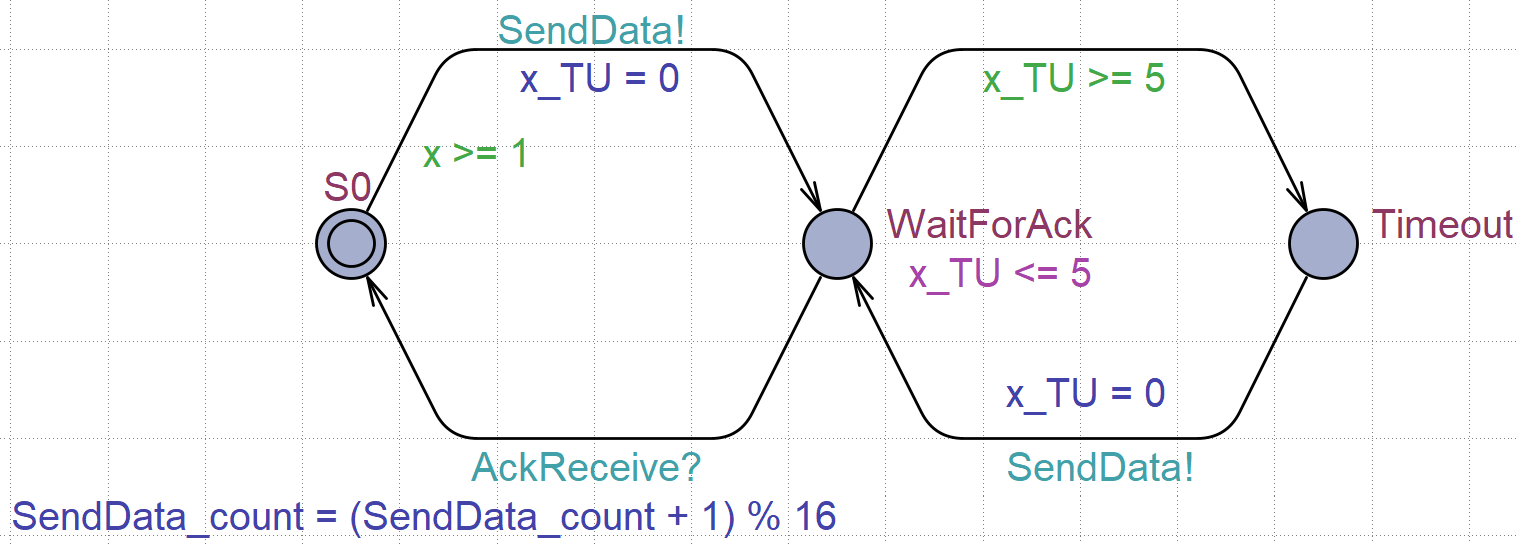
\includegraphics[width=0.8\textwidth]{images/Sender.png}
        \caption{}
        \label{fig:sender}
    \end{figure}

    \subsection*{Medium}
    The medium will receive the message at \textit{M0}, the message will then be transmitted to the receiver by sending the \textit{ReceiveData!}. If the medium receives an acknowledgement from the receiver, it will send the \textit{AckReceive!} to the sender. If the transmission is failed the medium will just go back to \textit{M0} and send nothing.

    \begin{figure}[H]
        \centering
        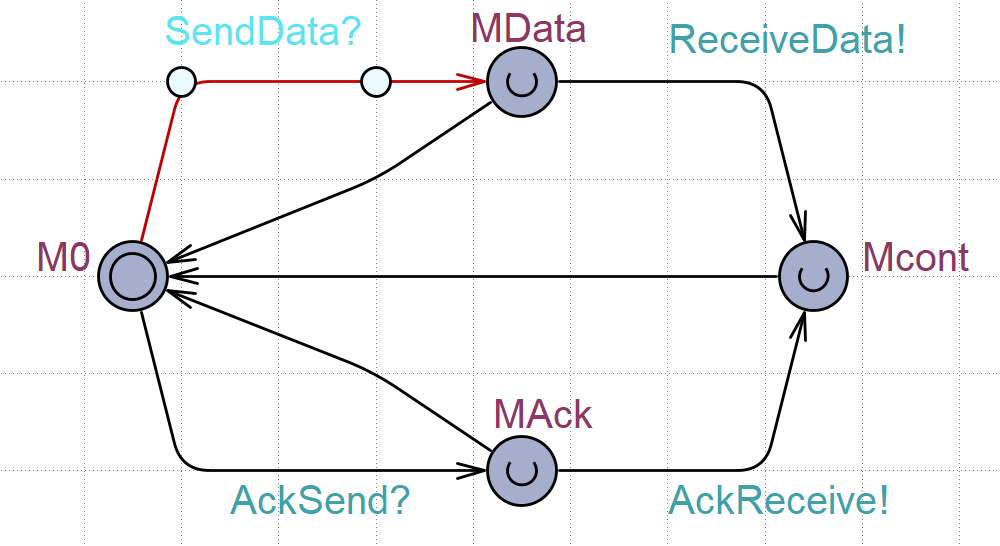
\includegraphics[width=0.6\textwidth]{images/Medium.png}
        \caption{}
        \label{fig:medium}    
    \end{figure}

    \subsection*{Receiver}
    The receiver will receive the message at \textit{R0}, it will then go to \textit{R\_receive} where it will acknowledge the transmission and sending an ack back to \textit{R0} which will then be picked up by the medium. If a loss of transmission occurs, the receiver will go to \textit{loss} and halt the system.

    \begin{figure}[H]
        \centering
        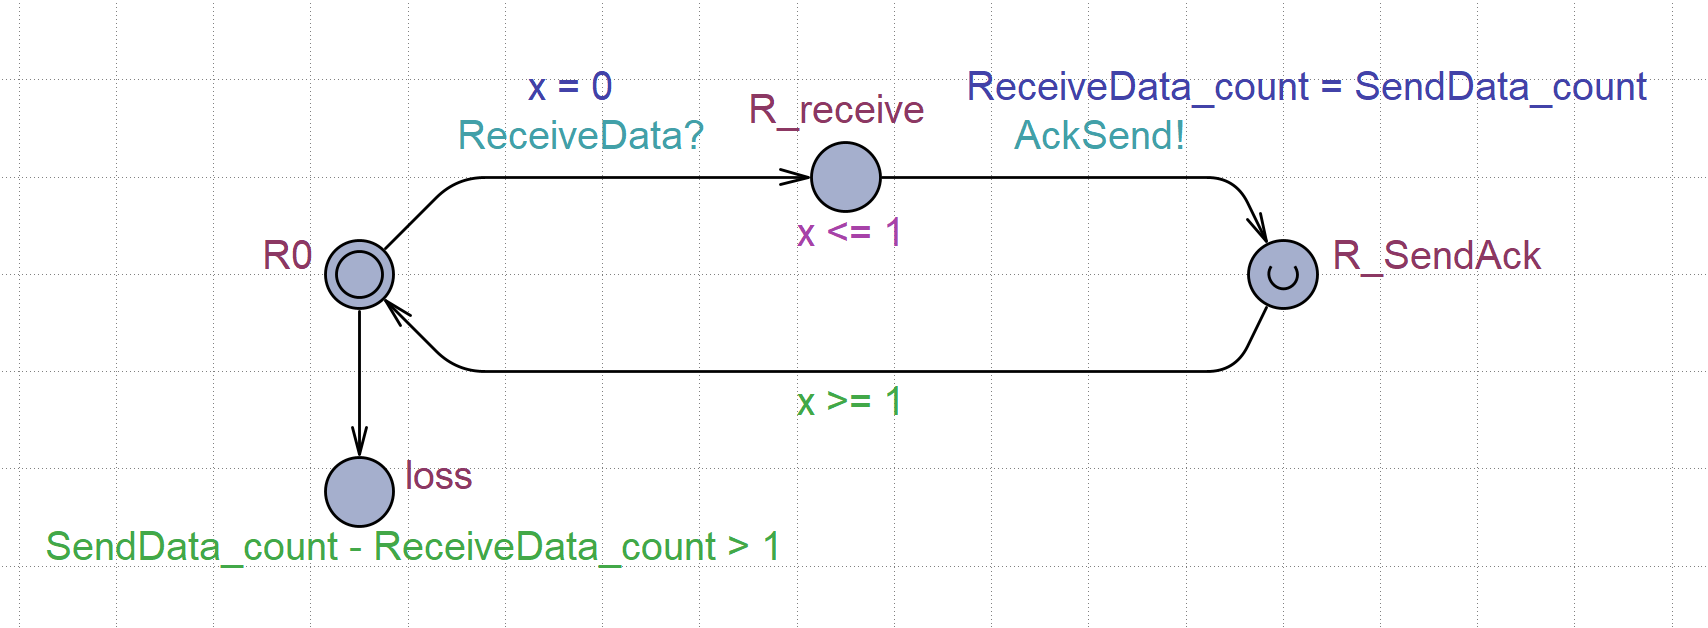
\includegraphics[width=0.8\textwidth]{images/Receiver.png}
        \caption{}
        \label{fig:receiver}    
    \end{figure}

    \subsection*{Verification}
    The verification is done using the commands in figure \ref{fig:verify}, the result in the first line shows that the system is deadlock free, the second line shows that the receiver will eventually receive the sent message to then send an acknowledgement and the third line shows that a loss of message never occurs since the message will always eventually be received.
    
    \begin{figure}[H]
        \centering
        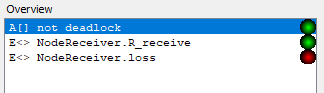
\includegraphics[width=0.6\textwidth]{images/Verify.png}
        \caption{}
        \label{fig:verify}    
    \end{figure}